\subsection{Радиус дуги окружности}
Самый простой и быстрый способ определения радиуса дуги окружности состоит в следующем. Необходимо построить хорду $AB$ максимальной длины: при угловой мере дуги меньше $180^\circ$~--- просто соединить концы дуги, больше~--- оптимальным будет провести хорду, близкую к диаметру. Затем, нужно провести серединный перпендикуляр $HH'$ к уже построенной хорде.

\begin{figure}[h!]
	\begin{subcaptionblock}[b]{0.5\tw}
		\centering
		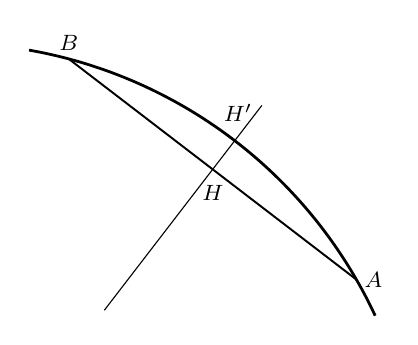
\begin{tikzpicture}
			\footnotesize
			\draw [line width=1pt] (5.44, 2.54) arc(25:80:6);
			\draw [line width=.7pt] (5.2, 3) -- (1.55, 5.8);
			
			\draw (2, 2.61) -- (4, 5.21);
			
			\point (5.2, 3);
			\point (1.55, 5.8);
			\point (3.38, 4.4);
			\point (3.65 , 4.76);
			
			\draw (5.2, 3) node [anchor=west] {$A$};
			\draw (1.55, 5.8) node [anchor=south] {$B$};
			\draw (3.38, 4.3) node [anchor=north] {$H$};
			\draw (3.7 , 4.9) node [anchor=south] {$H'$};
		\end{tikzpicture}
		\caption{}
		\label{pic:arc-radius-1}
	\end{subcaptionblock}
	\hfill
	\begin{subcaptionblock}[b]{0.5\tw}
		\centering
		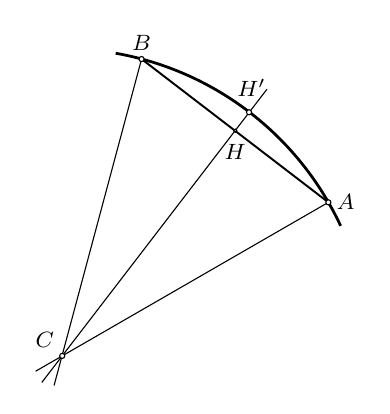
\begin{tikzpicture}[scale=0.65]
			\footnotesize
			\draw [line width=1pt] (5.44, 2.54) arc(25:80:6);
			\draw [line width=.7pt] (5.2, 3) -- (1.55, 5.8);
			\draw (-.4, -.52) -- (4, 5.21);
			\draw (-.52, -.3) -- (5.2, 3);
			\draw (-.16, -.58) -- (1.55, 5.8);
			
			\draw (5.2, 3) [fill=white] circle(.05);
			\draw (1.55, 5.8) [fill=white] circle(.05);
			\draw (3.38, 4.4) [fill=white] circle(.03);
			\draw (3.65 , 4.76) [fill=white] circle(.05);
			\draw (0, 0) [fill=white] circle(.05);
			
			\draw (5.2, 3) node [anchor=west] {$A$};
			\draw (1.55, 5.8) node [anchor=south] {$B$};
			\draw (3.38, 4.3) node [anchor=north] {$H$};
			\draw (3.7, 4.9) node [anchor=south] {$H'$};
			\draw (0, 0) node [anchor=south east] {$C$};
		\end{tikzpicture}
		\caption{}
		\label{pic:arc-radius-2}
	\end{subcaptionblock}
	\caption{}
\end{figure}

С помощью линейки можно измерить длину $l$ хорды $AB$~--- и длину $h$ отрезка перпендикуляра $HH'$, соединяющего $H$~--- точку пересечения с хордой,  и $H'$~--- точку пересечения с окружностью (см.~Рис.\,\ref{pic:arc-radius-1}). Если мысленно продолжить серединный перпендикуляр, то он, очевидно, пройдет через центр окружности $C$, а значит, в одной точке (в центре) пересечется с радиусами $AC$ и $BC$, проведенными в концы хорды (см.~Рис.\,\ref{pic:arc-radius-2}). Пусть~$r$~--- искомый радиус дуги, тогда из теоремы Пифагора получаем следующее:
\begin{gather*}
	(r - h)^2 = r^2 - \left( \frac{l}{2} \right)^2,\\
	r^2 - 2rh + h^2 = r^2 - \frac{l^2}{4},\\
	r = \frac{4h^2 + l^2}{8h}.
\end{gather*}

Аналогичный результат можно получить из теоремы об отрезках секущих, из которой следует, что
\begin{equation*}
	\frac{l}{2} \cdot \frac{l}{2} = (2r - h) \cdot h.
\end{equation*}

\begin{wrapfigure}[15]{r}{0.55\tw}
	\centering
	\vspace{-1.5pc}
	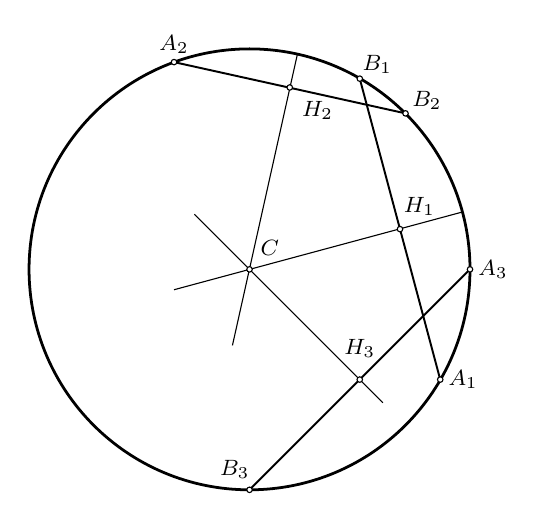
\begin{tikzpicture}[scale=0.7]
		\footnotesize
		\draw (0, 0) [line width=1pt] circle (4);
		\draw [line width=.7pt] (3.46, -2) -- (2, 3.46);
		\draw [line width=.7pt] (-1.37, 3.76) -- (2.83, 2.83);
		\draw [line width=.7pt] (4, 0) -- (0, -4);
		
		\draw (2.42, -2.42) -- (-1, 1);
		\draw (3.86, 1.04) -- (-1.37, -0.37);
		\draw (0.87, 3.91) -- (-0.31, -1.38);
		
		\draw (0, 0) [fill=white] circle(.05);
		\draw (2.73, 0.73) [fill=white] circle(.05);
		\draw (0.73, 3.3) [fill=white] circle(.05);
		\draw (2, -2) [fill=white] circle(.05);
		\draw (3.46, -2) [fill=white] circle(.05);
		\draw (2, 3.46) [fill=white] circle(.05);
		\draw (-1.37, 3.76) [fill=white] circle(.05);
		\draw (2.83, 2.83) [fill=white] circle(.05);
		\draw (4, 0) [fill=white] circle(.05);
		\draw (0, -4) [fill=white] circle(.05);
		
		\draw (0.05, 0.1) node[anchor=south west] {$C$};
		\draw (2.65, 0.83) node[anchor=south west] {$H_1$};
		\draw (0.8, 3.2) node[anchor=north west] {$H_2$};
		\draw (2, -1.75) node[anchor=south] {$H_3$};
		\draw (3.46, -2) node[anchor= west] {$A_1$};
		\draw (1.9, 3.4) node[anchor=south west] {$B_1$};
		\draw (-1.37, 3.76) node[anchor=south] {$A_2$};
		\draw (2.8, 2.75) node[anchor=south west] {$B_2$};
		\draw (4, 0) node[anchor= west] {$A_3$};
		\draw (0.15, -3.95) node[anchor=south east] {$B_3$};
	\end{tikzpicture}
	\caption{}
	\label{pic:arc-radius-chords}
\end{wrapfigure}
Однако для некоторых задач недостаточно величины радиуса дуги, необходимо знание положения центра окружности данной дуги. Для этого, например, можно воспользоваться предыдущим методом и найти радиус окружности, а потом отложить отрезок данной длины вдоль серединного перпендикуляра от точки пересечения с окружностью.

Но существует и другой способ. Можно провести две непараллельные хорды окружности и построить их серединные перпендикуляры. Так как они обязательно проходят через центр окружности~--- значит он будет точкой пересечения серединных перпендикуляров к хордам. В связи с возможными погрешностями при построениях рекомендуется строить не две, а три или четыре хорды и серединные перпендикуляры к ним (см.~Рис.\,\ref{pic:arc-radius-chords}). Критерием правильности и достаточной точности всех построений будет служить тот факт, что все серединные перпендикуляры к хордами пересеклись в одной точке.

Используя данный метод, очевидно, можно найти и радиус дуги (окружности), измерив расстояние от найденного  центра до произвольной точки на дуге (окружности) с помощью линейки.

